%%================================================
%% Filename: chap04.tex
%% Encoding: UTF-8
%% Author: 苏峻锋
%%================================================
\chapter{基于时间卷积网络的综合负载指标的预测}
在服务器集群的运作过程当中,因应访问时间及任务类型的不同,集群在特定时间段内可能会呈现出忙碌状态,其中部分节点由于负载过重而变得繁忙,而其他节点则处于空闲状态。这种情况下的节点主要存在两种状态:高负载与低负载。位于低负载(或高负载)状态的节点,通过负载均衡器的调整,可以恢复至正常负载状态。这种调节不仅能提高集群的整体资源使用效率,还能减轻高负载节点的运作压力。因此,本节内容通过探讨时间卷积网络的应用,旨在预测集群内服务器的综合负载情况,进而达到均衡每个服务器节点之间负载分配的目的。研究开始阶段,首先会通过探索通用的Linux系统来收集必要的数据。

\section{重要的负载指标的获取}
动态负载均衡算法的负载性能会受到服务器负载指标选取的影响。选择合适的负载信息生成合适的负载指标能够真实的反映服务器运行是的负载情况,
提升算法的准确度和动态负载均衡的负载效果。在第二章中已经知道了有哪些负载信息值得挑选和收集,但是没有一个真正的合适的负载综合指标来体现真实的负载情况。
具体的剩余性能的获取可以使用 Linux 的 proc 文件系统获取,该文件储存在内存里,不会占用外存的空间。

(1)CPU 信息的获取

要获取 Linux 系统中的 CPU 详细使用情况可以使用 cat/proc/stat,CPU 详细使用情况如下表。

\begin{longtblr}[
	caption = {CPU 详细信息解释},
	]{
	width = \linewidth,
	colspec = {Q[102]Q[837]},
	vline{2} = {-}{},
	hline{1,9} = {-}{0.08em},
			hline{2} = {-}{},
		}
	参数      & 解释                           \\
	user    & 用户态 CPU 时间,高优先级的进程           \\
	system  & 操作系统内核所占用的CPU时间              \\
	idle    & CPU处于空闲状态的时间总和,不包括等待硬盘I/O的时间 \\
	iowait  & CPU因等待硬盘输入输出操作而处于空闲的时间       \\
	irq     & 处理硬件中断所花费的CPU时间              \\
	softirq & 处理软件中断所花费的CPU时间
\end{longtblr}

那么 CPU 利用率的计算公式为:$CPU_{usg} = 1 - (idle_2 - idle_1) / (cpu_2 - cpu_1)$ 通过使用 cat /proc/cpuinfo 命令获取服务器 CPU 配置,然后在 benchmark 上可纯到该 CPU 性能的分数作为 $CPU_{mark}$。则一个节点的 CPU 的剩余性能如下。
\begin{align}
	C_{j}=(1-CPU_{usg_{j}})\frac{n^{\ast}CPU_{mark_{j}}}{\sum_{1}^{n}CPU_{mark}}
\end{align}

(2) 内存信息获取
获取内存使用情况则可以 cat /proc/meminfo 命令,其中最重要的是 MemFree、Buffers、Cached 三个信息分别是完全空闲的内存大小、缓存文件系统的元数据和跟踪正在读写的块设备、存储页缓存和slabs的内存大小。所以内存使用率的计算方式如下。
\begin{equation}
	MEM_{usg} = (1 - MemFree + Buffers + Cached) / MemFree
\end{equation}

(3)磁盘信息获取

磁盘信息可以通过 iostat -x /dev/sda1  命令获取。重要信息如下表。

% \usepackage{tabularray}
\begin{longtblr}[
	caption = {磁盘信息获取},
	]{
	width = \linewidth,
	colspec = {Q[81]Q[860]},
	hlines,
	vlines,
	hline{1,8} = {-}{0.08em},
		}
	标示~     & 说明                                                 \\
	Device~ & 监测设备名称                                             \\
	rkB/s~  & 每秒实际读取的大小,单位为KB                                    \\
	wkB/s~  & 每秒实际写入的大小,单位为KB                                    \\
	await~  & 等待I/O平均的时间(milliseconds)                           \\
	svctm~  & I/O需求完成的平均时间                                       \\
	\%util~ & 设备带宽的使用率,达到100\%表示饱和,达到性能瓶颈,如果是支持处理并发请求的设备则不代表性能瓶颈
\end{longtblr}

(4)网络带宽信息获取

使用命令 cat /proc/net/dev 获取网络数据,并记录一定时间内的接收(Receive)和发送(Transmit)字节(bytes)的变化量,从而计算出网络口的传输速率$T_{bytes}$ 网络带宽记为 Bandwidth,带宽使用率定义为:$NET_{usg} = T_{bytes} / Bandwidth$

在获取关键性能指标后,进一步构建综合性的负载评价指标至关重要。为了客观计算服务器节点的当前负载,本文提出一个综合负载决策模型,该模型将各单项负载指标进行综合。其中,加权和法由于在构建服务器负载状态模型中展现的优势,往往被采用。传统研究中,权重系数通常基于经验设定,而本文提倡采用主成分分析法(PCA)以科学地确定权重系数向量,从而提升服务器响应精确性和可靠性。

主成分分析法(Principal Componet Analysis, PCA)最早是由 Pearson\cite{kpfrs1901lines}提出的一种多变量统计分析方法,
该方法通过正交变换将原始数据转换成一组由线性无关变量变量表示的数据,以达到数据降维的目的\cite{李可佳2023基于主成分分析和函数机制的差分隐私线性回归算法}。具体步骤如下。

已经收集了服务器节点的 CPU 利用率、内存利用率、设备 IO 使用率,和带宽使用率的数据,将这些数据保存在以个表中,每一列代表一个指标,每一行代表一个观测时间点的数据。
由于主成分分析法的要求,将不同的特征量纲统一到相同的尺度,这样就可以公平地比较和组合这些特征,需要对给定数据集进行标准化。
对于每个指标,计算所有数据点的均值。公式为:$\mu=\frac{1}{N}\sum_{i=1}^{N}x_{i}$ 其中$\mu$ 为均值,N 是观测的个数,$x_{i}$ 每个观测的值。
计算标准差:然后计算每个指标的标准差。公式为:$\sigma = \sqrt{\frac{1}{N} \sum_{i = 1}^{N} \left(\right. x_{i} - \mu \left(\left.\right)\right)^{2}\frac{\sigma}{2}}$其中$\sigma$是标准差。
最后进行Z-score标准化:对每个指标的每个数据点进行标准化,公式为 $z = \frac{(x_{i} - \mu)}{\sigma}$ 其中 $z$ 就是最后每个指标每个观测时间的标准化后的值。

给定标准化后的数据集 $X = [x_1, x_2, \cdots, x_n]^{\mathbf{T}} \in \mathbb{R}^{n \times d}$,其中 $n$ 为样本的数量,$d$ 指标的数量,
结合在一起,\( X \) 是一个由 \( n \) 个 \( d \)-维的实数向量构成的数据集,并且以矩阵形式表示,其中每一行是一个样本,每一列是一个特征。则数据集的协方差公式矩阵如下。
\begin{equation}
	A={\frac{1}{n}}X^{\mathsf{T}}X={\frac{1}{n}}\sum_{i\,=\,1}^{n}x_{i}x_{i}^{\mathsf{T}}=V\Sigma V^{\mathsf{T}}\in\mathbb{R}^{d\cdot d}
\end{equation}

对 $\mathbf{A}$ 进行特征分解后得到一组降序排列的特征值$\lambda_1 \ge \lambda_2 ... \ge \lambda_n > 0$ 相对应的单位特征向量 $v_1, v_2, \dots, v_n$。
其中,特征值越大的,其对应的主成分越重要。于是,综合负载决策函数如下。
\begin{equation}
	\mathbf{X} = \mu_1C_{usg} + \mu_2M_{usg} + \mu_3D_{usg} + \mu_4N_{usg}
\end{equation}

通过指定欲保留的主成分比重阈值 $\theta \in (0, 1]$ 来确定目标唯独 k 的大小。
具TCN 模型参数组合体来说$\k$可以通过 $\frac{\sum^{k}_{i = 1}\lambda_i}{\sum^{d}_{i = 1}\lambda_i} \ge \theta$ 来得到。
取前 $k$ 个特征值对应的特征向量组成的主成分空间$\mathbb{V}_{d \times k} = (v_1, v_2, \cdots, v_k)$。将标准化后的原始数据集$\mathbf{X}_{n \times d}$ 投影到由前 $k$ 个特征向量构成的主成分空间 $\mathbf{V}_{d \times k}$中,得到了降维后的 $k$ 维数据集。
\begin{equation}
	\mathbf{Z}_{n \times k} = \mathbf{X}_{n \times d}\mathbf{V}_{d \times k}
\end{equation}

在这个公式中,$\mathbf{X}_{n \times d}$ 表示标准化后的原始数据集,其中 $n$ 是样本数,$d$ 是原始特征数。$\mathbf{V}_{d \times k}$ 包括了前 $k$ 个特征值对应的特征向量(这些特征向量通常是按照特征值大小从大到小排列的),它们构成了主成分空间。这个空间的维度($k$)通常远小于原始特征空间的维度($d$)。

当原始数据集 $\mathbf{X}$ 与主成分空间 $\mathbf{V}_{d \times k}$ 相乘时,得到的 $\mathbf{Z}_{n \times k}$ 就是投影到这个 $k$ 维空间的数据集。在这个 $k$ 维空间中,每一行代表了原始数据的一个样本,每一列则对应一个主成分。$\mathbf{Z}$ 的列向量提供了在主成分空间中的坐标,即降维后的数据表示。

其中在进行特征分解后,就已经得到了主成分空间,空间内含有了最重要的4个特征值,
这个特征值就是权重的系数,通过降维与原始数据值相乘后得到的就是每个指标乘以权重系数后的数据集,只需要对降维的数据集进行每一列的相加,即可对得到时间序列-综合负载指标的数据集。

\section{时间卷积网络的关键特征}
时间卷积网络由传统的 CNN 改进的专门处理时间序列的深度学习模型\cite{lea2016temporal}。一开始认为,时序问题(如语言、语音等等)天生就是 RNN 的地盘。然而现在这一观点要成为过去式了。时间卷积网络(Temporal Convolutional Nets, TCNs)作为 CNN 家族中的一员健将,拥有许多新特性,如今已经在诸多主要应用领域中击败了 RNN。看起来 RNN 可能要成为历史了。

卷积神经网络(Convolutional Neural Nets, CNNs)是在图像和视频识别领域公认的核心工具,与此类似,循环神经网络(Recurrent Neural Nets, RNNs)在自然语言处理领域中也扮演了同样关键的角色。
然而, CNN 和 RNN 的主要差别在于,CNN 崭露头角的领域是静态图像(或视图区分为帧)的识别, RNN 则在需处理序列或时间依赖问题的文本和语音方面大放异彩。
这也就形成了一种情况:字母或词汇的预测依赖于其前面的字母或词汇,从而引入了时间的概念,并考虑到序列的特点。
实际上,RNN 在所有序列问题上,包括语音/文本识别、机器翻译、手写体识别、序列数据分析(预测)以及各种配置下的自动编码生成等都表现出色。
然而,RNN 的问题在于其计算密度极高,因为在整个任务完成之前必须保存所有的中间结果,且深度神经网络在前一个单词处理完之前都不能进行下一个单词的处理。
因此,TCN(Temporal Convolutional Networks)应运而生。

时间卷积网络需要的数据集和RNN 有一定的类似,在处理时间序列数据集时都要进行嵌入(Embedding)操作。Embedding的主要目的是将时序数据映射到一个稠密的连续向量空间中,使得相似的语义信息在该向量空间中也能够彼此接近。这样,神经网络就可以基于这些向量表示学习到输入数据的复杂语义信息,并在相似的向量表示之间进行泛化。图是具体的嵌入过程。

\begin{figure}[htbp]
	\centering
	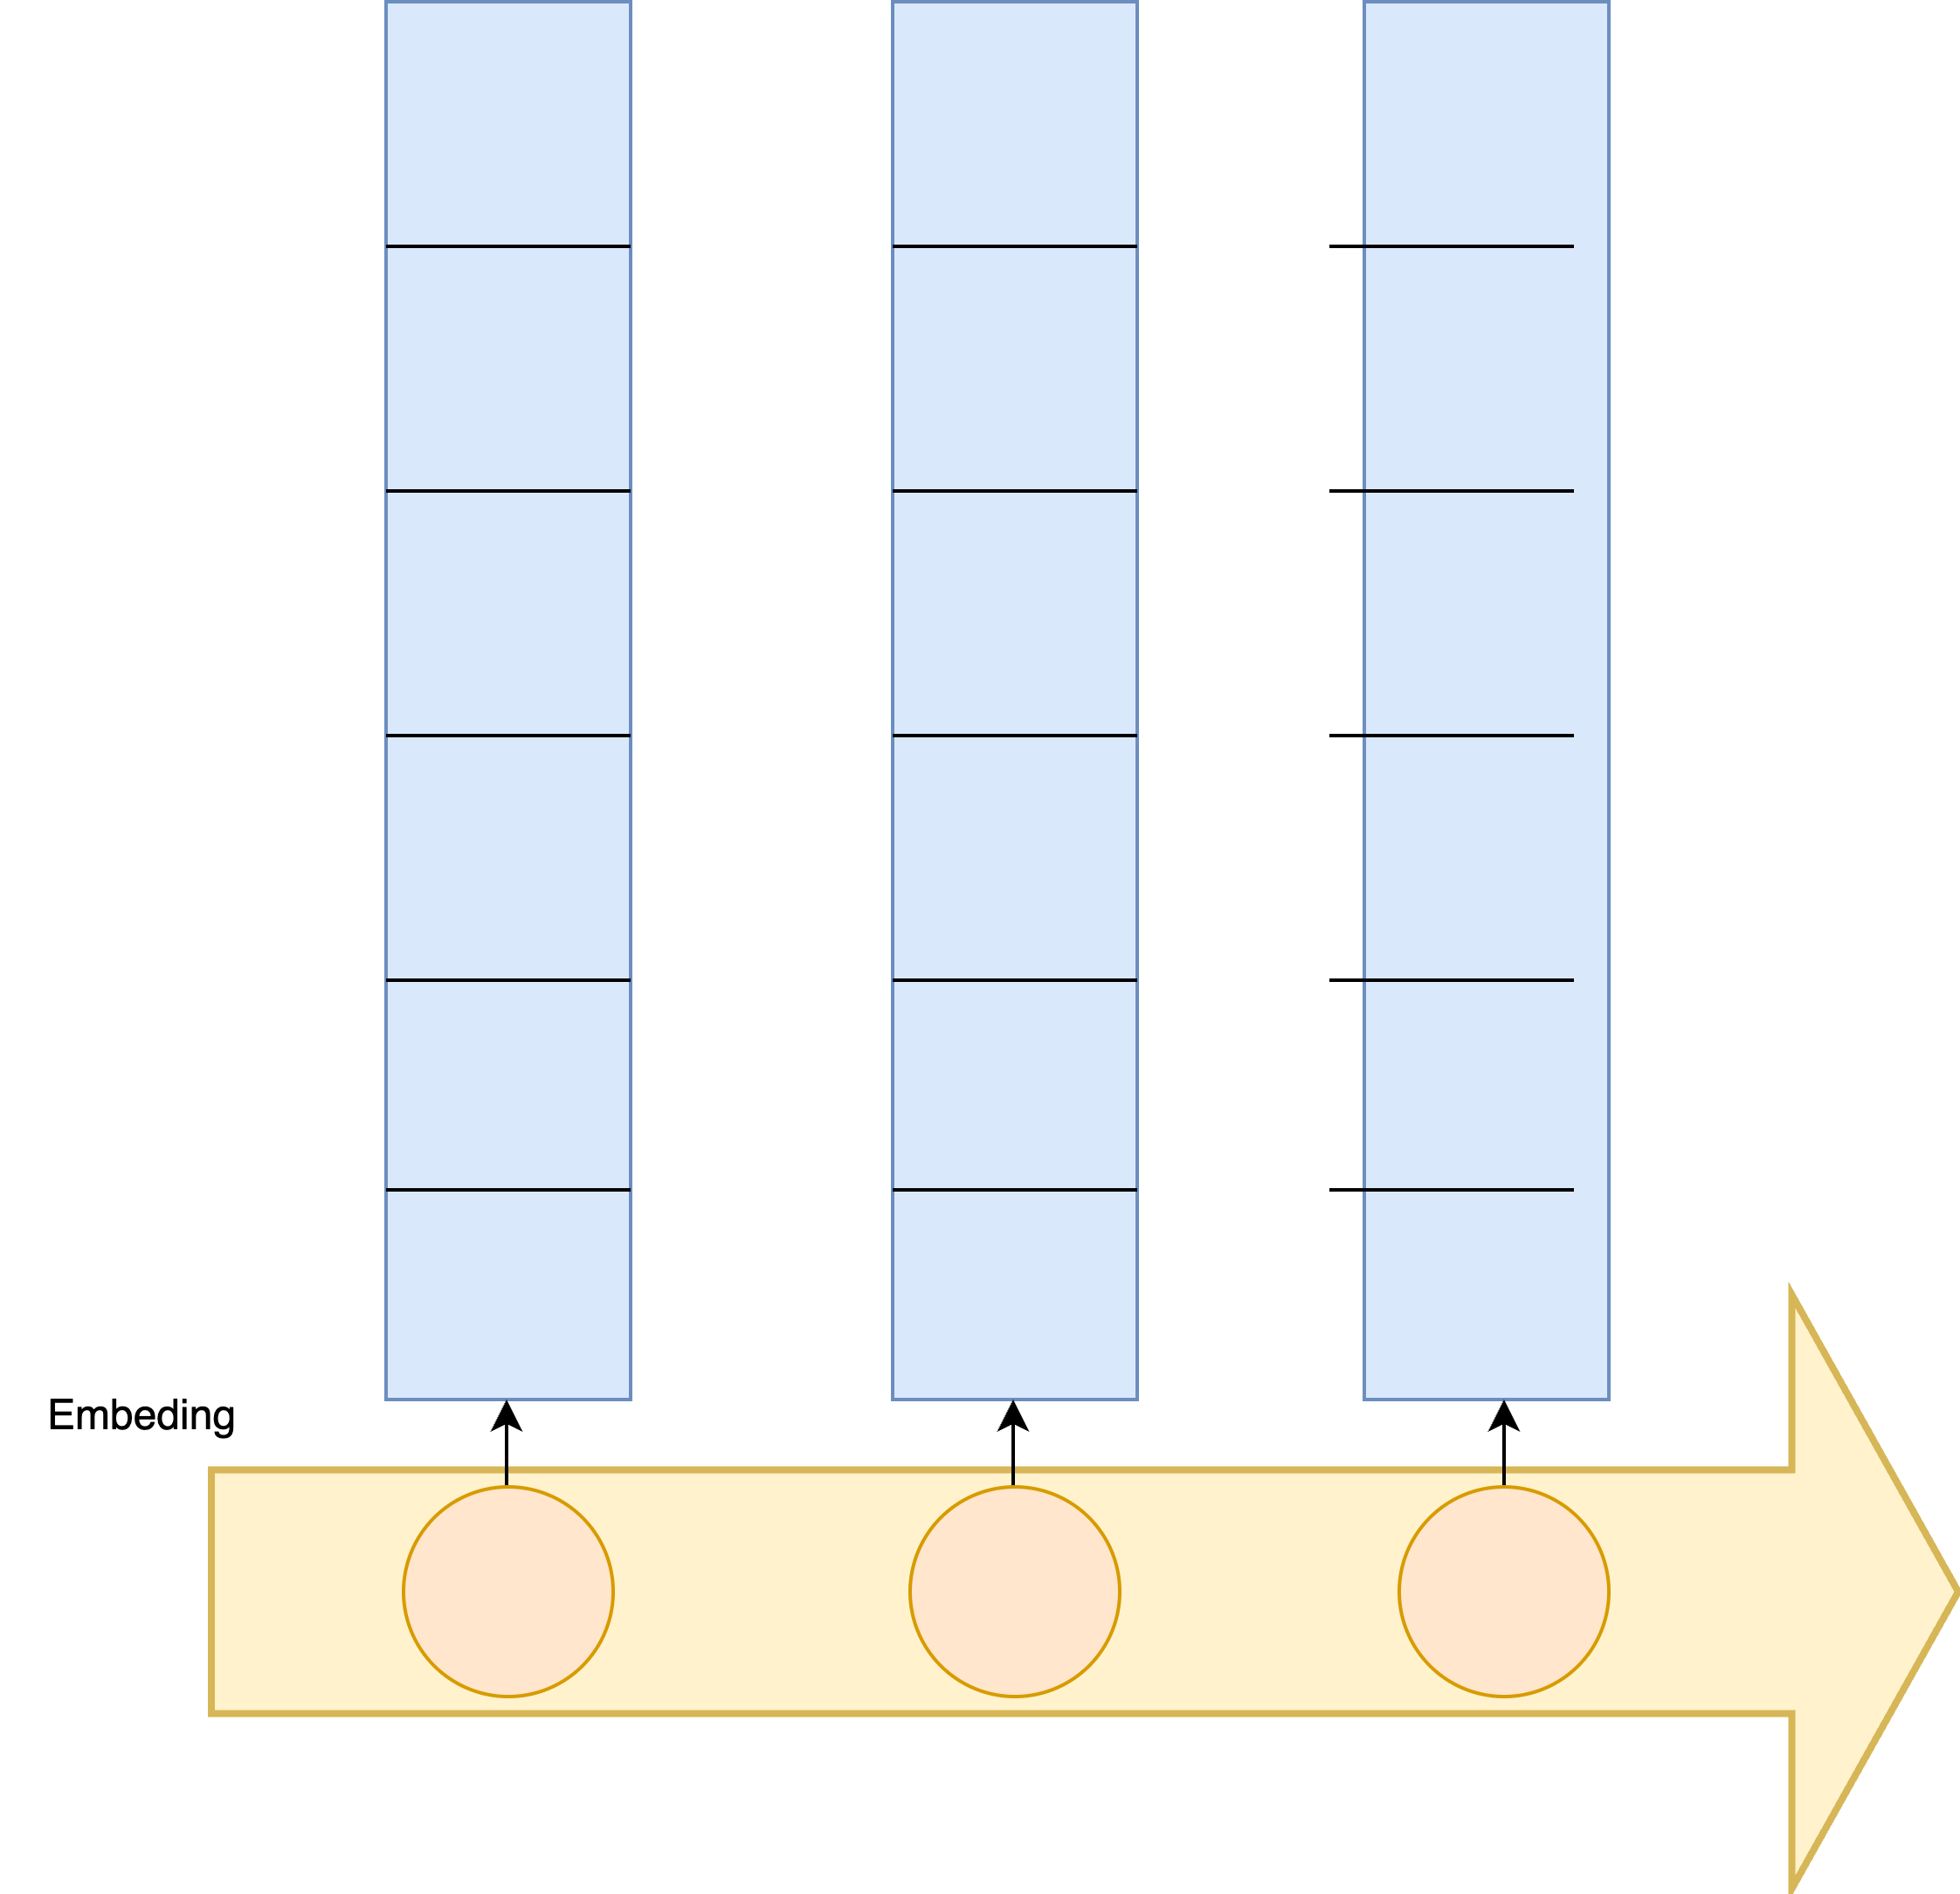
\includegraphics[width=0.7\textwidth]{figures/embedding.png}
	\caption{原始时序序列嵌入生成向量}
\end{figure}

TCN所依赖的卷积操作在本质上就是一维卷积(1D-CNN)。一维卷积利用多个大小固定的卷积核与输入序列进行卷积运算来生成输出序列。卷积核的形状由输入通道数$in\_channels$ 和卷积核大小$kernel\_size$ 共同决定,卷积核的数量则由输出通道数$out\_channels$决定。
经过Embedding后的时序数据的通道数由1扩展成了$embedding\_size$ ,对于有着 $in\_channels$ 个通道的时序数据作为输入, 一维卷积使用 $out\_channels$ 个大小为($in\_channels, kernel\_size$)的卷积核进行卷积操作。

假设有一个时间序列,总共有五个时间点,比方说股市,有一个股票的价格波动:[10,13,12,14,15]。TCN 使用一个卷积大小为 2 的卷积核,对上面5个数据做一个卷积核大小为2的卷积是什么样子如下。

\begin{figure}[htbp]
	\centering
	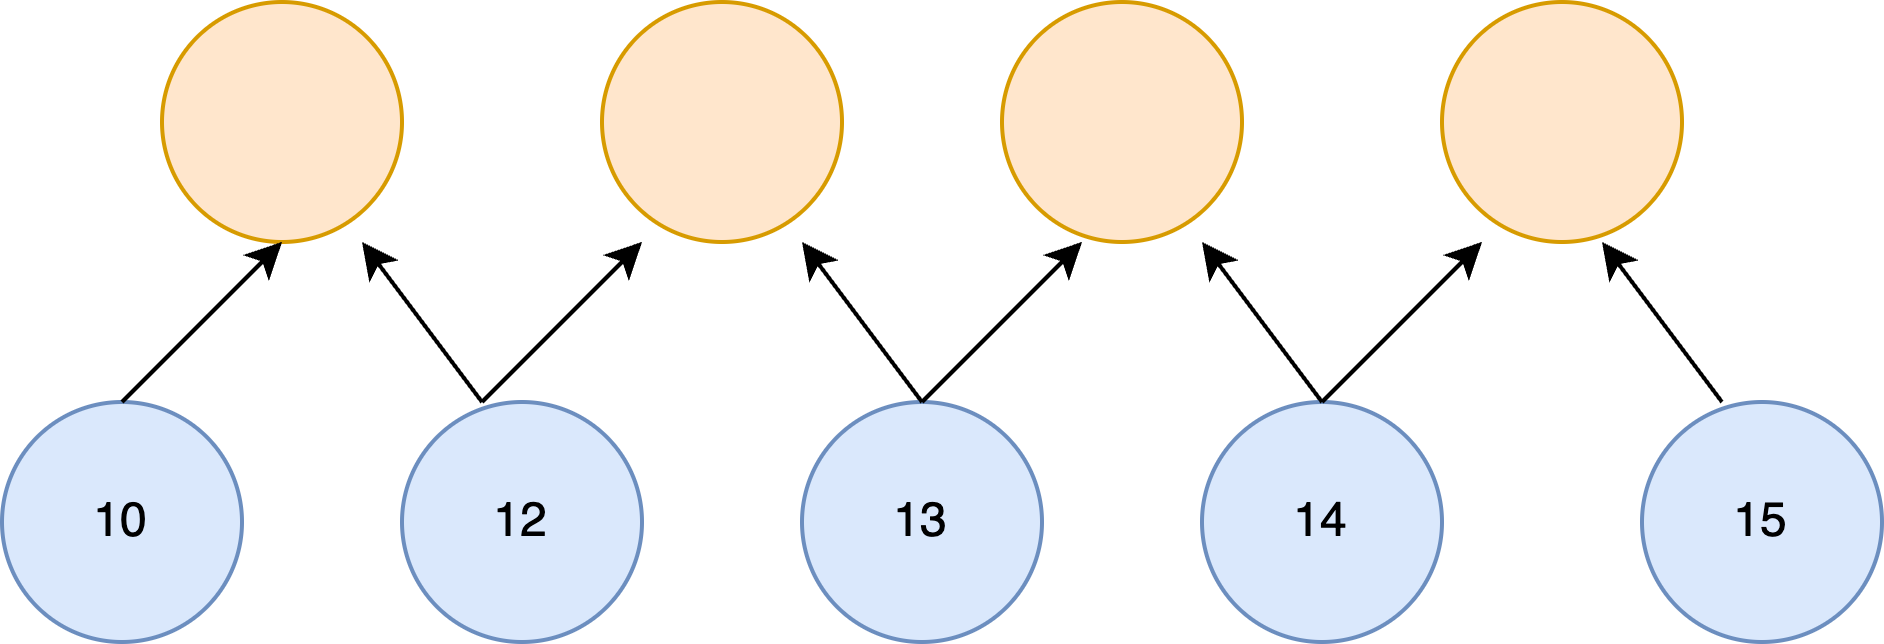
\includegraphics[width=.9\textwidth]{figures/convolution_1.png}
	\caption{卷积核为2的卷积过程}
\end{figure}

五个数据经过一次卷积,可以变成四个数据,
但是每一个卷积后的数据都是基于两个原始数据得到的,所以说,目前卷积的视野域是2。可以看到是输入是5个数据,但是经过卷积,变成4个数据了。TCN网络的第一个原则是输入和输出的形状必须相同。而在进行一维卷积操作时,假设第$i$ 层的输入长度为$L_i$ 卷积核大小为 $K$ 则输出长度为 $L_{i+1} = L_{i} - K + 1$。为满足这个原则,TCN在使用卷积神经网络进行序列处理时,通常需要进行 Padding 操作。通过在输入序列的左侧添加一定数量$K-1$ 的 0,实现信号维度的保持,使通过卷积和池化处理后的数据与输入数据的长度相同。在一维卷积中进行的Padding操作默认会在左右都进行填充,
所以TCN进行了额外的裁剪操作。

\begin{figure}[htbp]
	\centering
	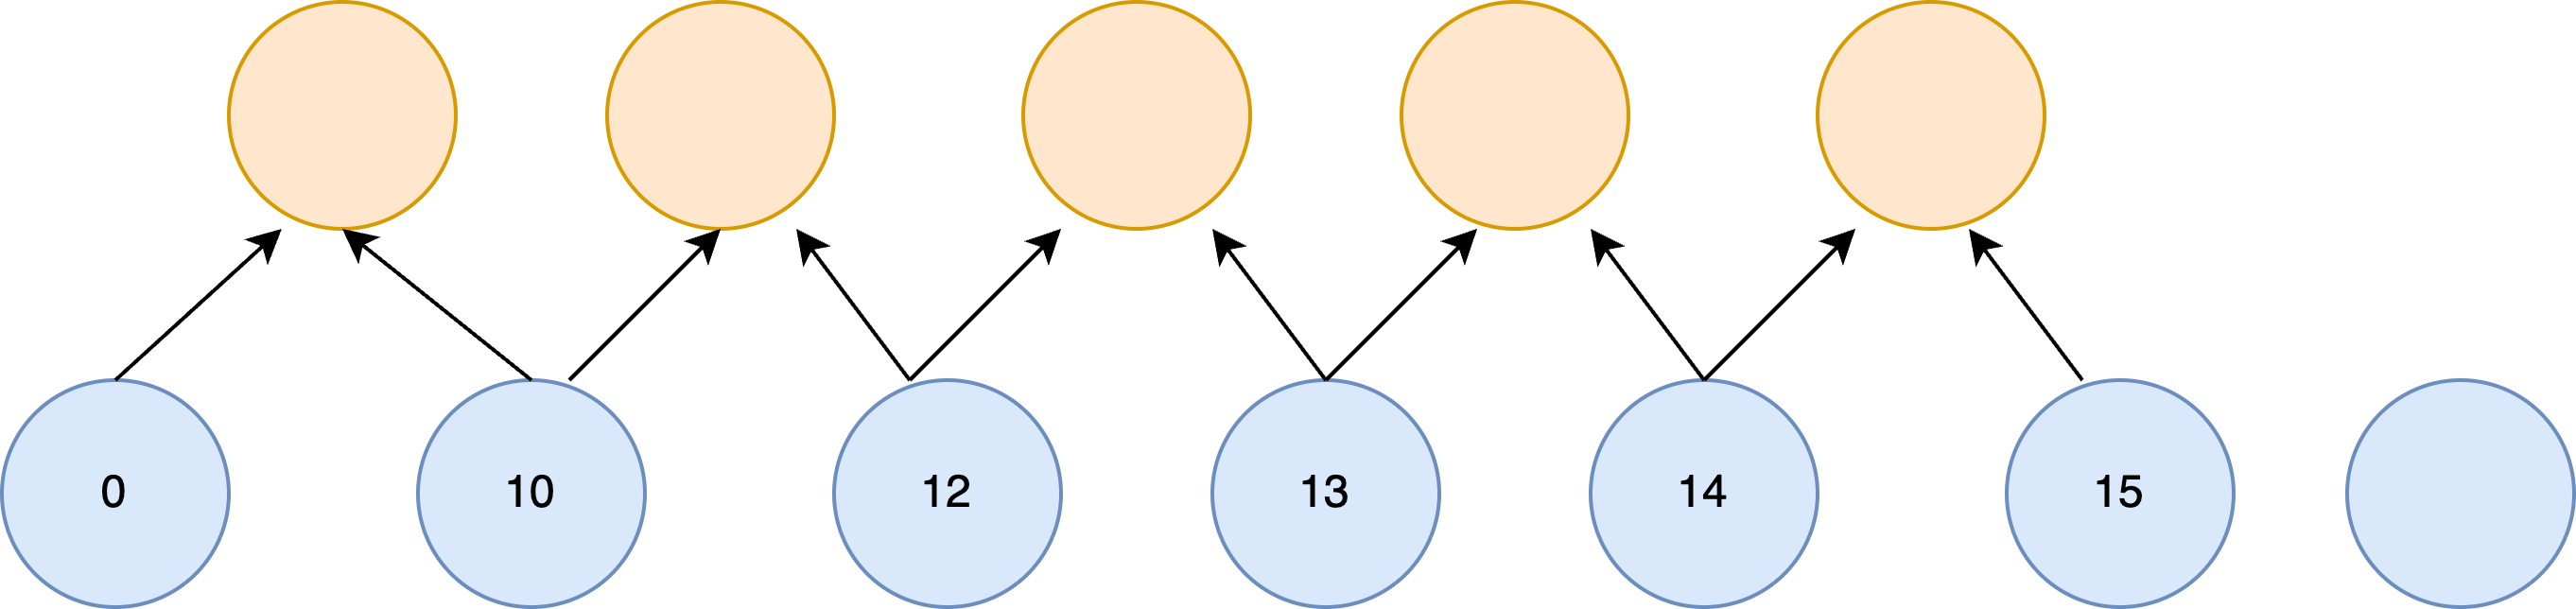
\includegraphics[width=0.9\textwidth]{figures/convolution_2.png}
	\caption{padding 后的卷积}
\end{figure}

padding是左右两头都增加0,如果padding是1的话,就是上图的效果,其实会产生6个新数据,但是秉着:“输入输出尺寸相同”和“我们不能知道未来的数据”,所以最后边那个未来的padding,就省略掉了,之后会在代码中会体现出来。

时间卷积网络有两个原则,其一就是上面的TCN 网络的输入和输出形状必须相同,以确保模型对时序数据的处理不会丢失信息。其二,TCN 网络中的每一时刻的输出仅由该时刻及其之前的输入卷积得到,以确保其在处理序列时具有因果约束。
通过使用因果卷积满足原则二,因果卷积是一种只考虑过去时间状态的一维卷积操作。因果卷积的具体步骤如下图所示。

\begin{figure}[htbp]
	\centering
	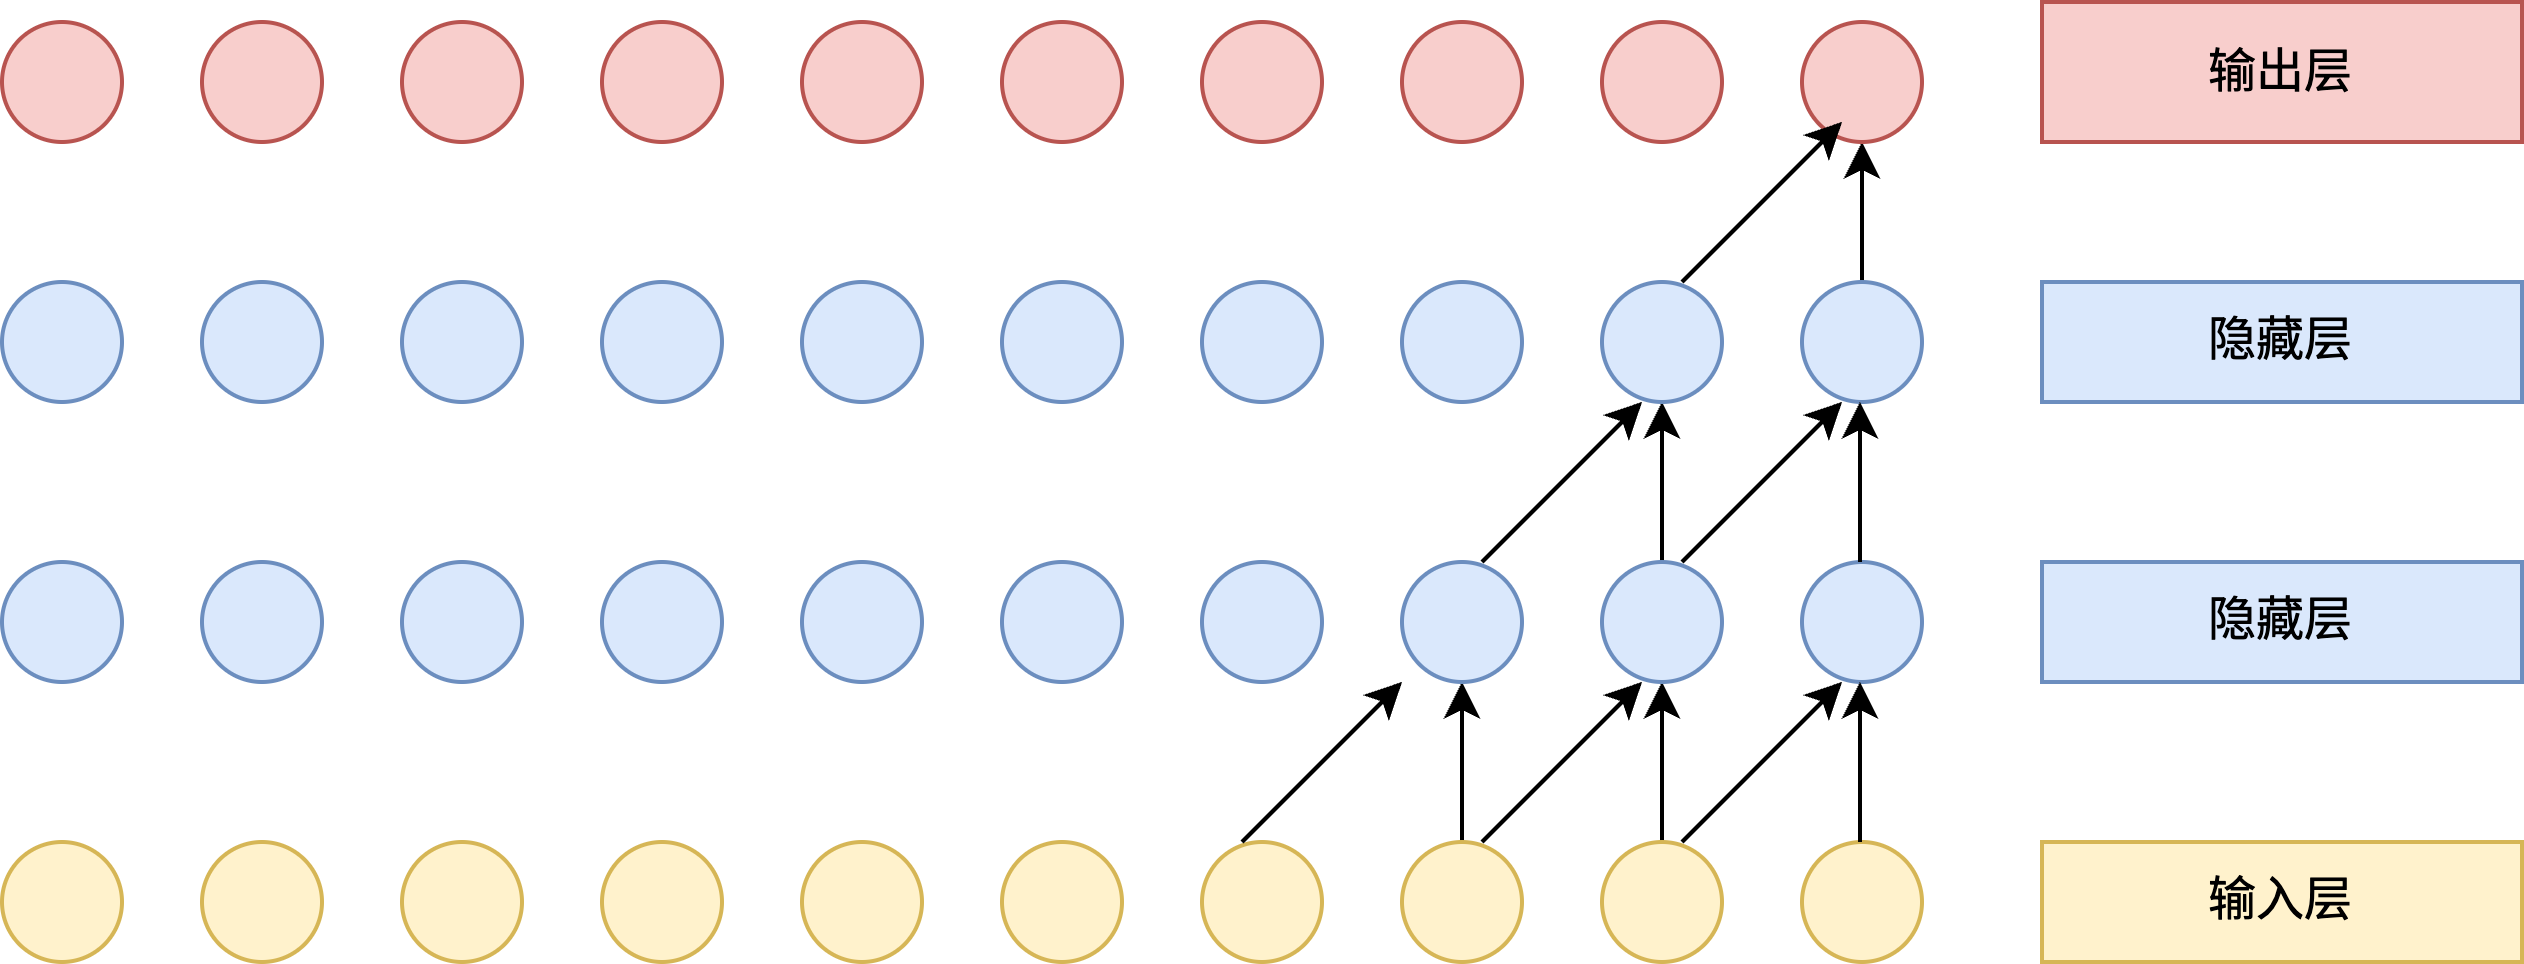
\includegraphics[width=\textwidth]{figures/causal_convolution.png}
	\caption{因果卷积}
\end{figure}

图中可以看到,因果卷积具备了两个特点。只考虑过去的信息。 时刻的输出$y_t$ 仅依赖于 $x_0\text{,} \dots \text{,}x_t$ ,而不依赖任何“未来”的输入$x_{t+1} \text{,} \dots \text{,}x_T$。
同时追溯历史信息越久远,隐藏层越多。 图中,输出层期望采集输入层的4个时间步,则需要2个隐藏层。而业务的需求往往要求采取更多的时间步,确实是“深度”学习了。

由于因果卷积没有循环连接,它们通常比循环神经网络(RNN)训练速度更快,尤其是应用于非常长的序列。
但是,针对于一般的时间序列而言,往往是按照分钟记录的,那少说也是十万、百万的数据量,想要考虑之前1000个时间点呢?视野域要是1000,那意味着要999层卷积。
每经过一层,节点相对于前层减少一个,我们最后的输出只有一个节点,如果输入视野为1000,需要经过999层才能变为最后输出的一个节点。
啥计算机吃得消这样的计算。所以引入了膨胀因果卷积。



传统的因果卷积面临对时间建模长度的局限,这个长度通常由卷积核的大小决定。要捕获更长的依赖关系需要通过线性堆积多个卷积层才能实现。然而,尽管标准CNN可以通过增加池化层来扩大感受野,但此举无疑会导致信息的损失。

膨胀卷积通过在标准卷积中引入"空洞"来增大感受野。与传统卷积不同,膨胀卷积允许卷积时对输入进行间隔采样,采样率由超参数dilation rate控制,表示卷积核中元素之间的下标间隔。引入"空洞"的好处在于,无需通过池化操作而损失信息,就可以扩大感受野,使每个卷积输出包含更大范围的信息。
当dilation rate等于2时,膨胀因果卷积的示意图展示了这一过程。通过在卷积核中注入"空洞",卷积操作可以跳过一些输入元素,覆盖更广的范围,同时保留因果性质,即当前输出仅依赖于当前时刻及之前的输入。这种方式能够以更少的参数和更少的层数建模长距离依赖,提升了时间序列建模的效率和精度。

\begin{figure}[htbp]
	\centering
	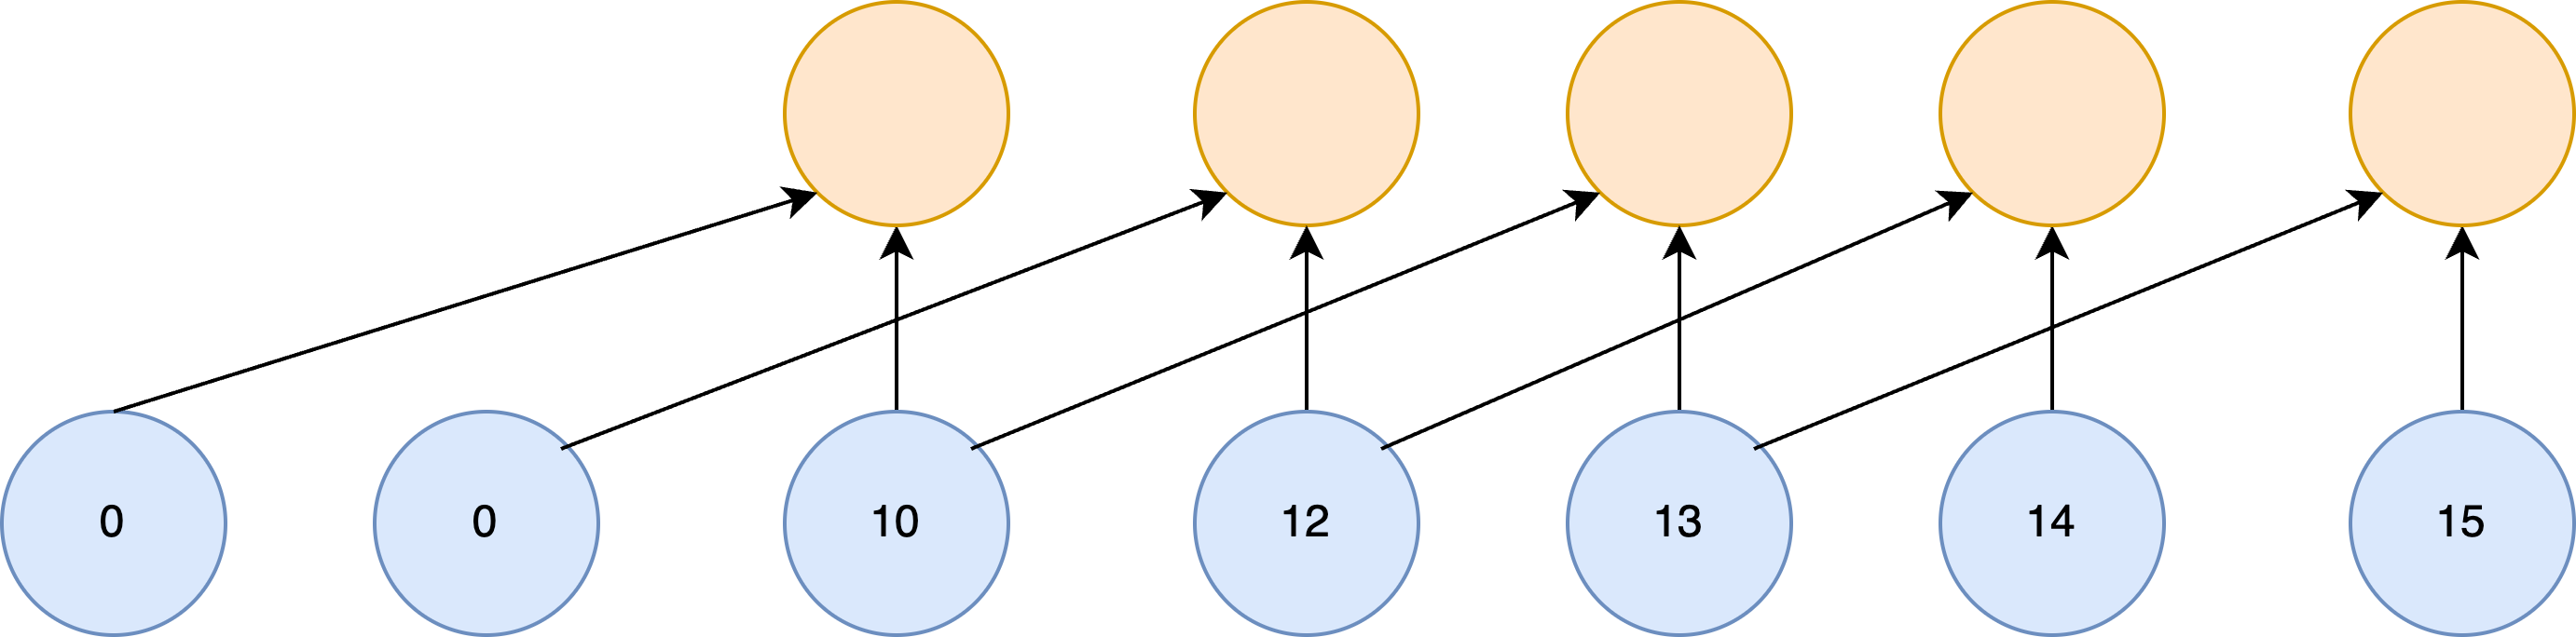
\includegraphics[width=\textwidth]{figures/dilation_convolution.png}
	\caption{dilation=2 的膨胀因果卷积}
\end{figure}

图中,可以看到卷积核大小依然是2,但是卷积核之间变得空洞了,每2个点采样一个作为输入;
如果dilation=3的话,那么可以想而知,这个卷积核中间会空的更大,每3个点采样一个作为输入。
因为dilation变大了,所以相应的padding的数量从1变成了2,所以为了保证输入输出的特征维度相同,
padding的数值在卷积核是2的情况下等于dalition的数值。
一般情况下,$padding=(kernel\_size-1)\times dilation$,每个卷积核元素之间有 $dilation - 1$ 个空洞节点,
所以空洞因果卷积的感受野范围大小为 $(kernel\_size-1) \times dilation + 1$。
以输入中的第一个元素作为空洞因果卷积的最后一个元素,则它的左边需要padding的个数为$(kernel\_size-1) \times dilation$。于是较为完备的 TCN 训练网络如下。

\begin{figure}[htbp]
	\centering
	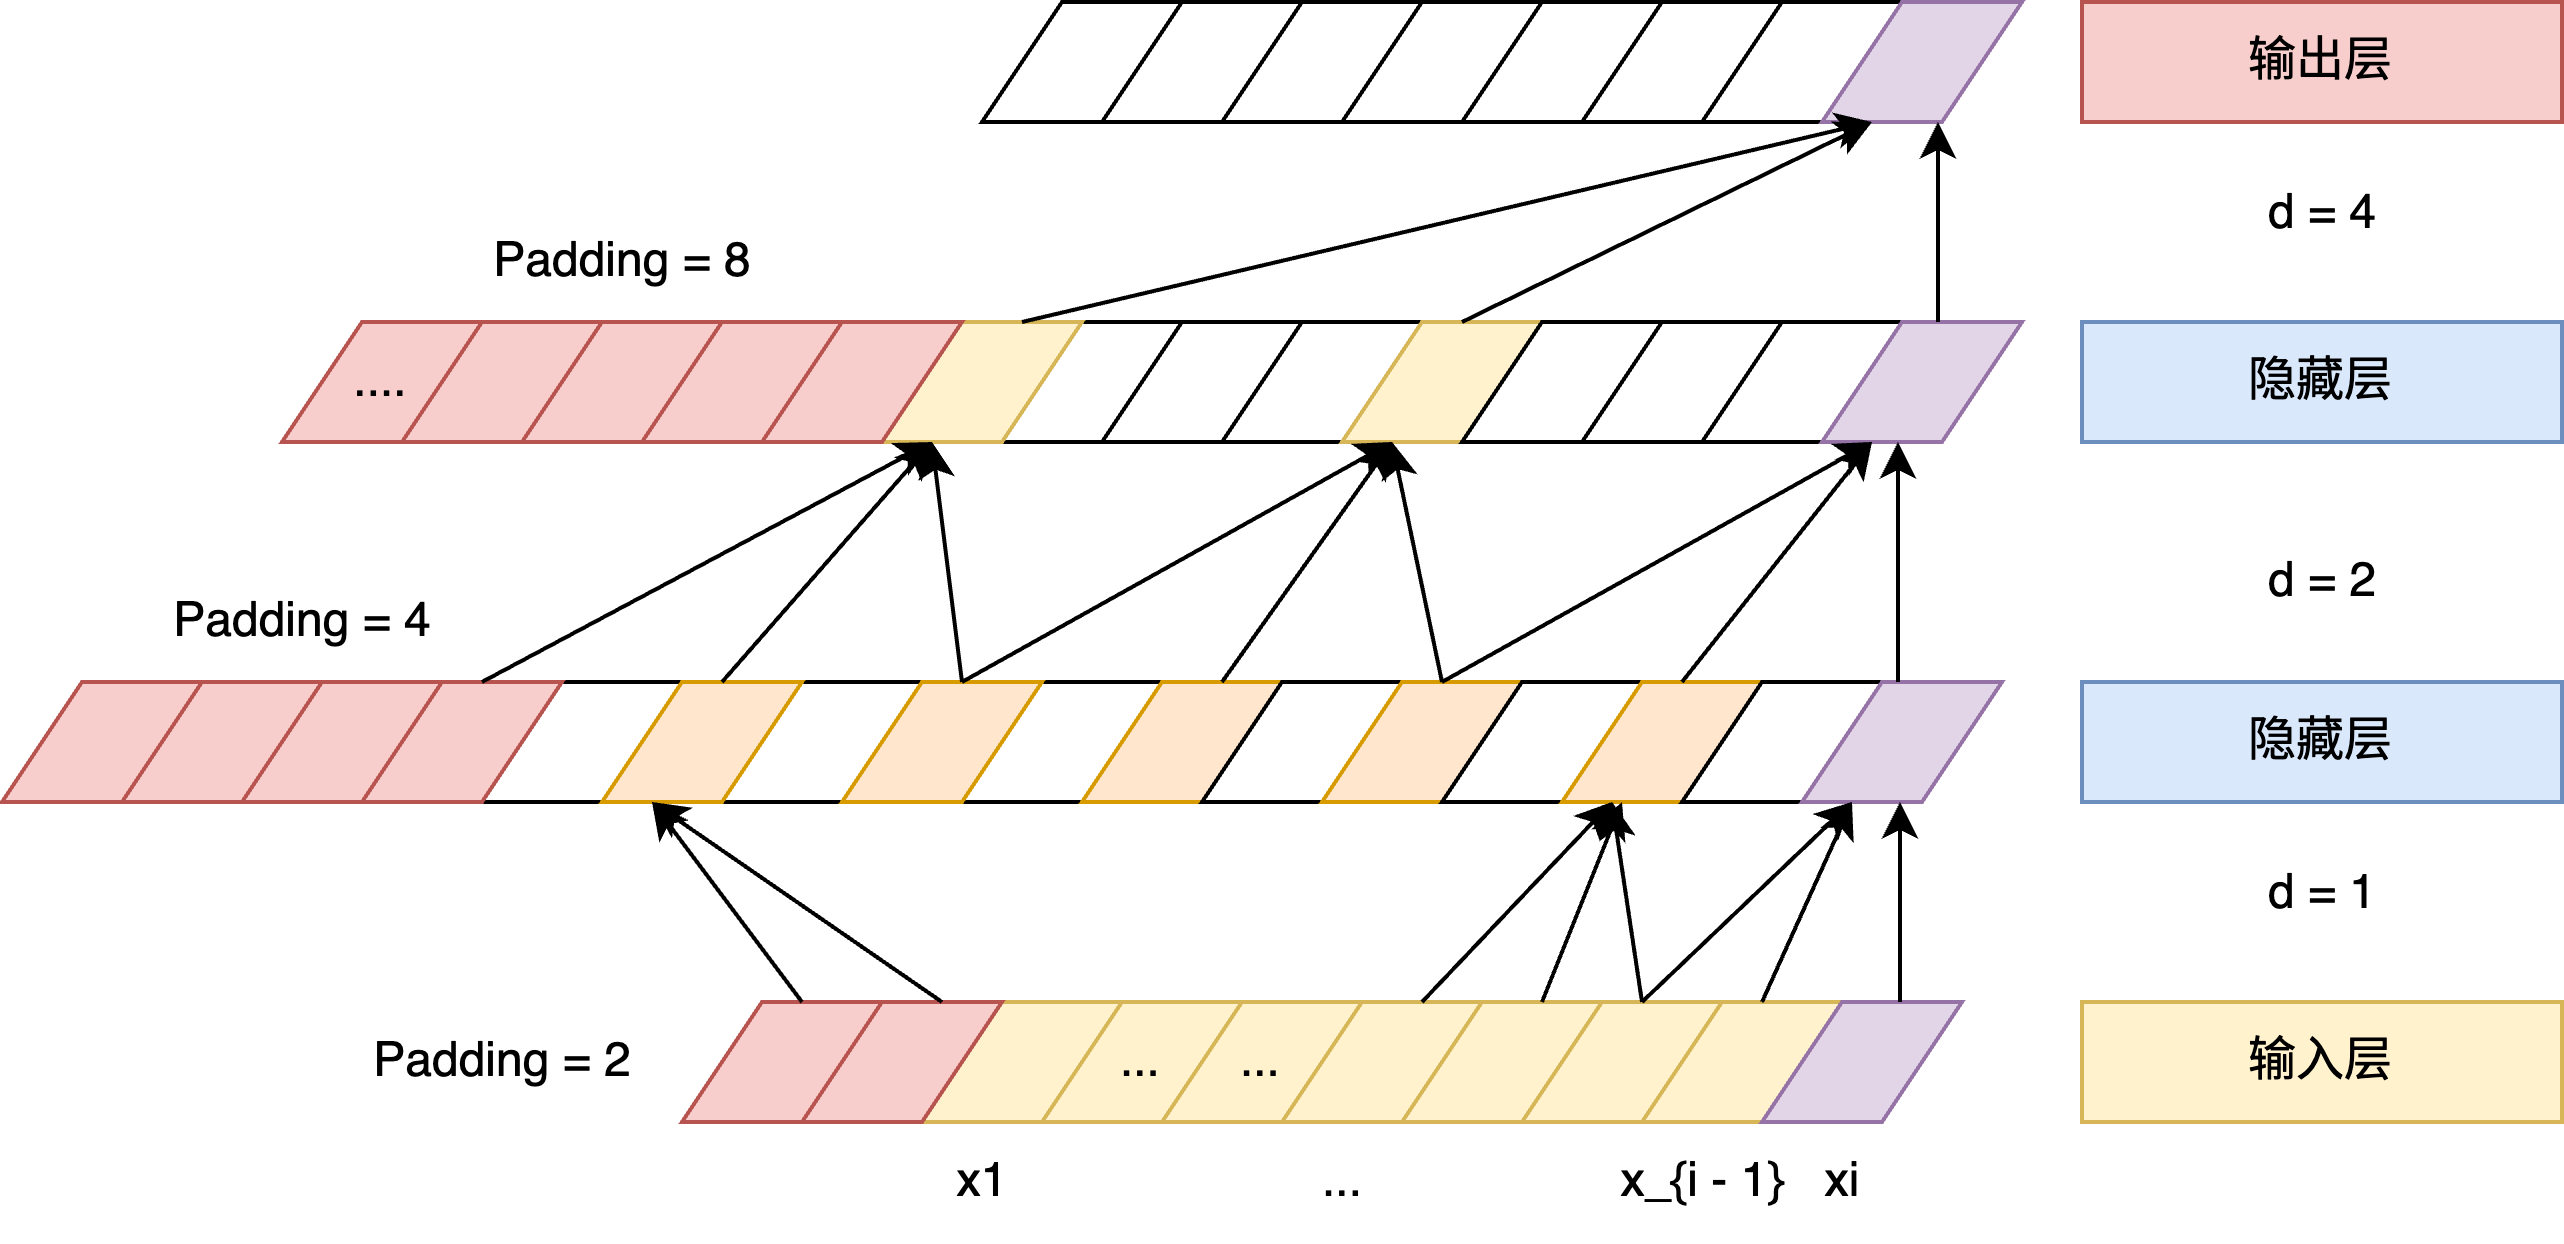
\includegraphics[width=\textwidth]{figures/tcn_1.png}
	\caption{TCN 训练网络骨干}
\end{figure}

从图中可以看到,每一层在时刻$t$的值,仅与其上一层在时刻$t, t-1, \dots$的值相关,这符合因果卷积的原理。此外,信息的提取过程在每一层中都是以跳跃式进行的,且每层的空洞率(dilated rate)都以2的指数形式增加,展现了空洞卷积的特点。同时,由于采纳了空洞卷积,每个隐藏层都需要进行填充(padding),其大小由公式$padding = (kernel\_size - 1)$确定。

深度卷积神经网络(CNN)通过其多层结构,能够捕获到不同层次的特征信息,层数越多,提取的特征越是抽象和高级。但是,仅仅增加网络的深度可能会遇到梯度消失或梯度爆炸的问题。尽管通过合适的权重初始化和增加正则化层可以在一定程度上缓解这一问题,使得训练多达数十层的网络成为可能。但随着网络层数的增加,网络退化的问题却随之而来\cite{吕国豪2014基于卷积神经网络的正则化方法}。

网络退化是指,尽管从理论上讲,高层次的网络结构包含了低层次的网络结构,但在使用随机梯度下降法进行训练时,往往只能找到局部最优解而非全局最优解。例如,虽然理论上最优的网络结构可能是18层,但在尝试设计34层的更深网络时,超出的16层可能实际上是多余的。理想情况下,我们希望模型在训练过程中能够自动把这16层转换为恒等映射,使得其输入与输出保持一致。然而,模型很难精确地学习这16层的恒等映射参数,导致34层网络的性能不如一个最优的18层网络。这就是网络加深过程中出现的模型退化问题。

因此,网络退化问题的解决关键在于使网络中的冗余层能够实现恒等映射,从而使得深层网络与浅层网络等效。为了达到这一目的,时间卷积网络引入了残差模块,成功地解决了网络退化问题。

\begin{figure}[htbp]
	\centering
	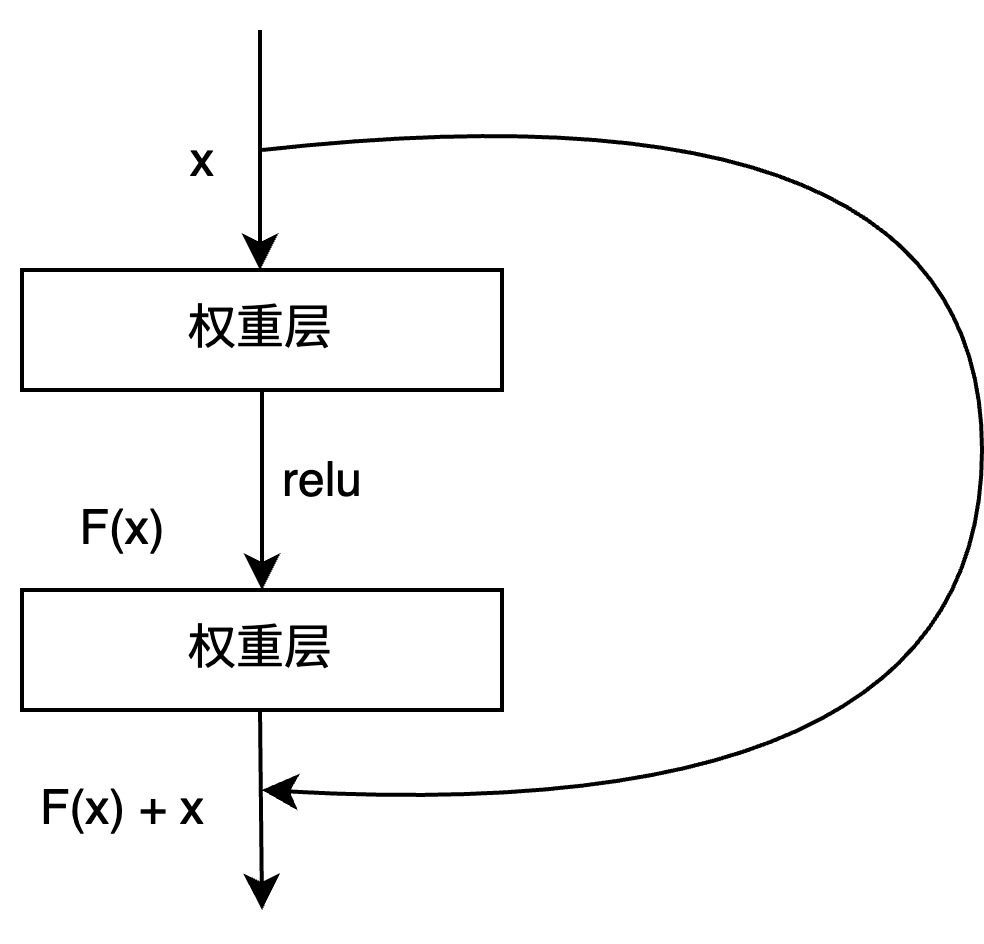
\includegraphics[width=0.5\textwidth]{figures/residual_block.png}
	\caption{残差模块}
	\label{residual_block}
\end{figure}

在通常情况下,要使网络层学习到恒等映射函数 $H(x) = x$ 是有一定难度的。但是,通过将网络函数定义为 $H(x) = F(x) + x$ 可以将恒等映射转化为残差函数 $F(x) = H(x) - x$。 这意味着,只要  $F(x) = 0$,就构成了一个恒等映射 $H(x) = x$。在图\ref{residual_block}中,
身份映射被称为shortcut连接,而残差映射对应 $F(x)$。残差网络的核心思想在于,如果网络达到了最优状态,进一步增加网络深度时,残差映射将被推向0,留下的只有身份映射。理论上,这保持了网络始终处于最优状态,从而网络的性能不会因深度增加而下降。

实验证明,残差模块往往需要两层以上,单单一层的残差模块 并不能起到提升作用\cite{he2016deep}。shortcut 连接有两种,如果是同等维度的映射则 $F(x)=W_2σ(W_1x+b_1)+b_2\text{,}H(x)=F(x)+x$,
如果维度不同则 $F(x)=W_2σ(W_1x+b_1)+b_2\text{,}H(x)=F(x)+W_sx$。虽然残差模块刚开始是基于全连接层的表示,实际上残差模块可以用于卷积层。加法变为 channel 间的两个 feature map 逐个元素相加。下图\ref{residual_tcn}是时间卷积网络的残差模块。

\begin{figure}[htbp]
	\centering
	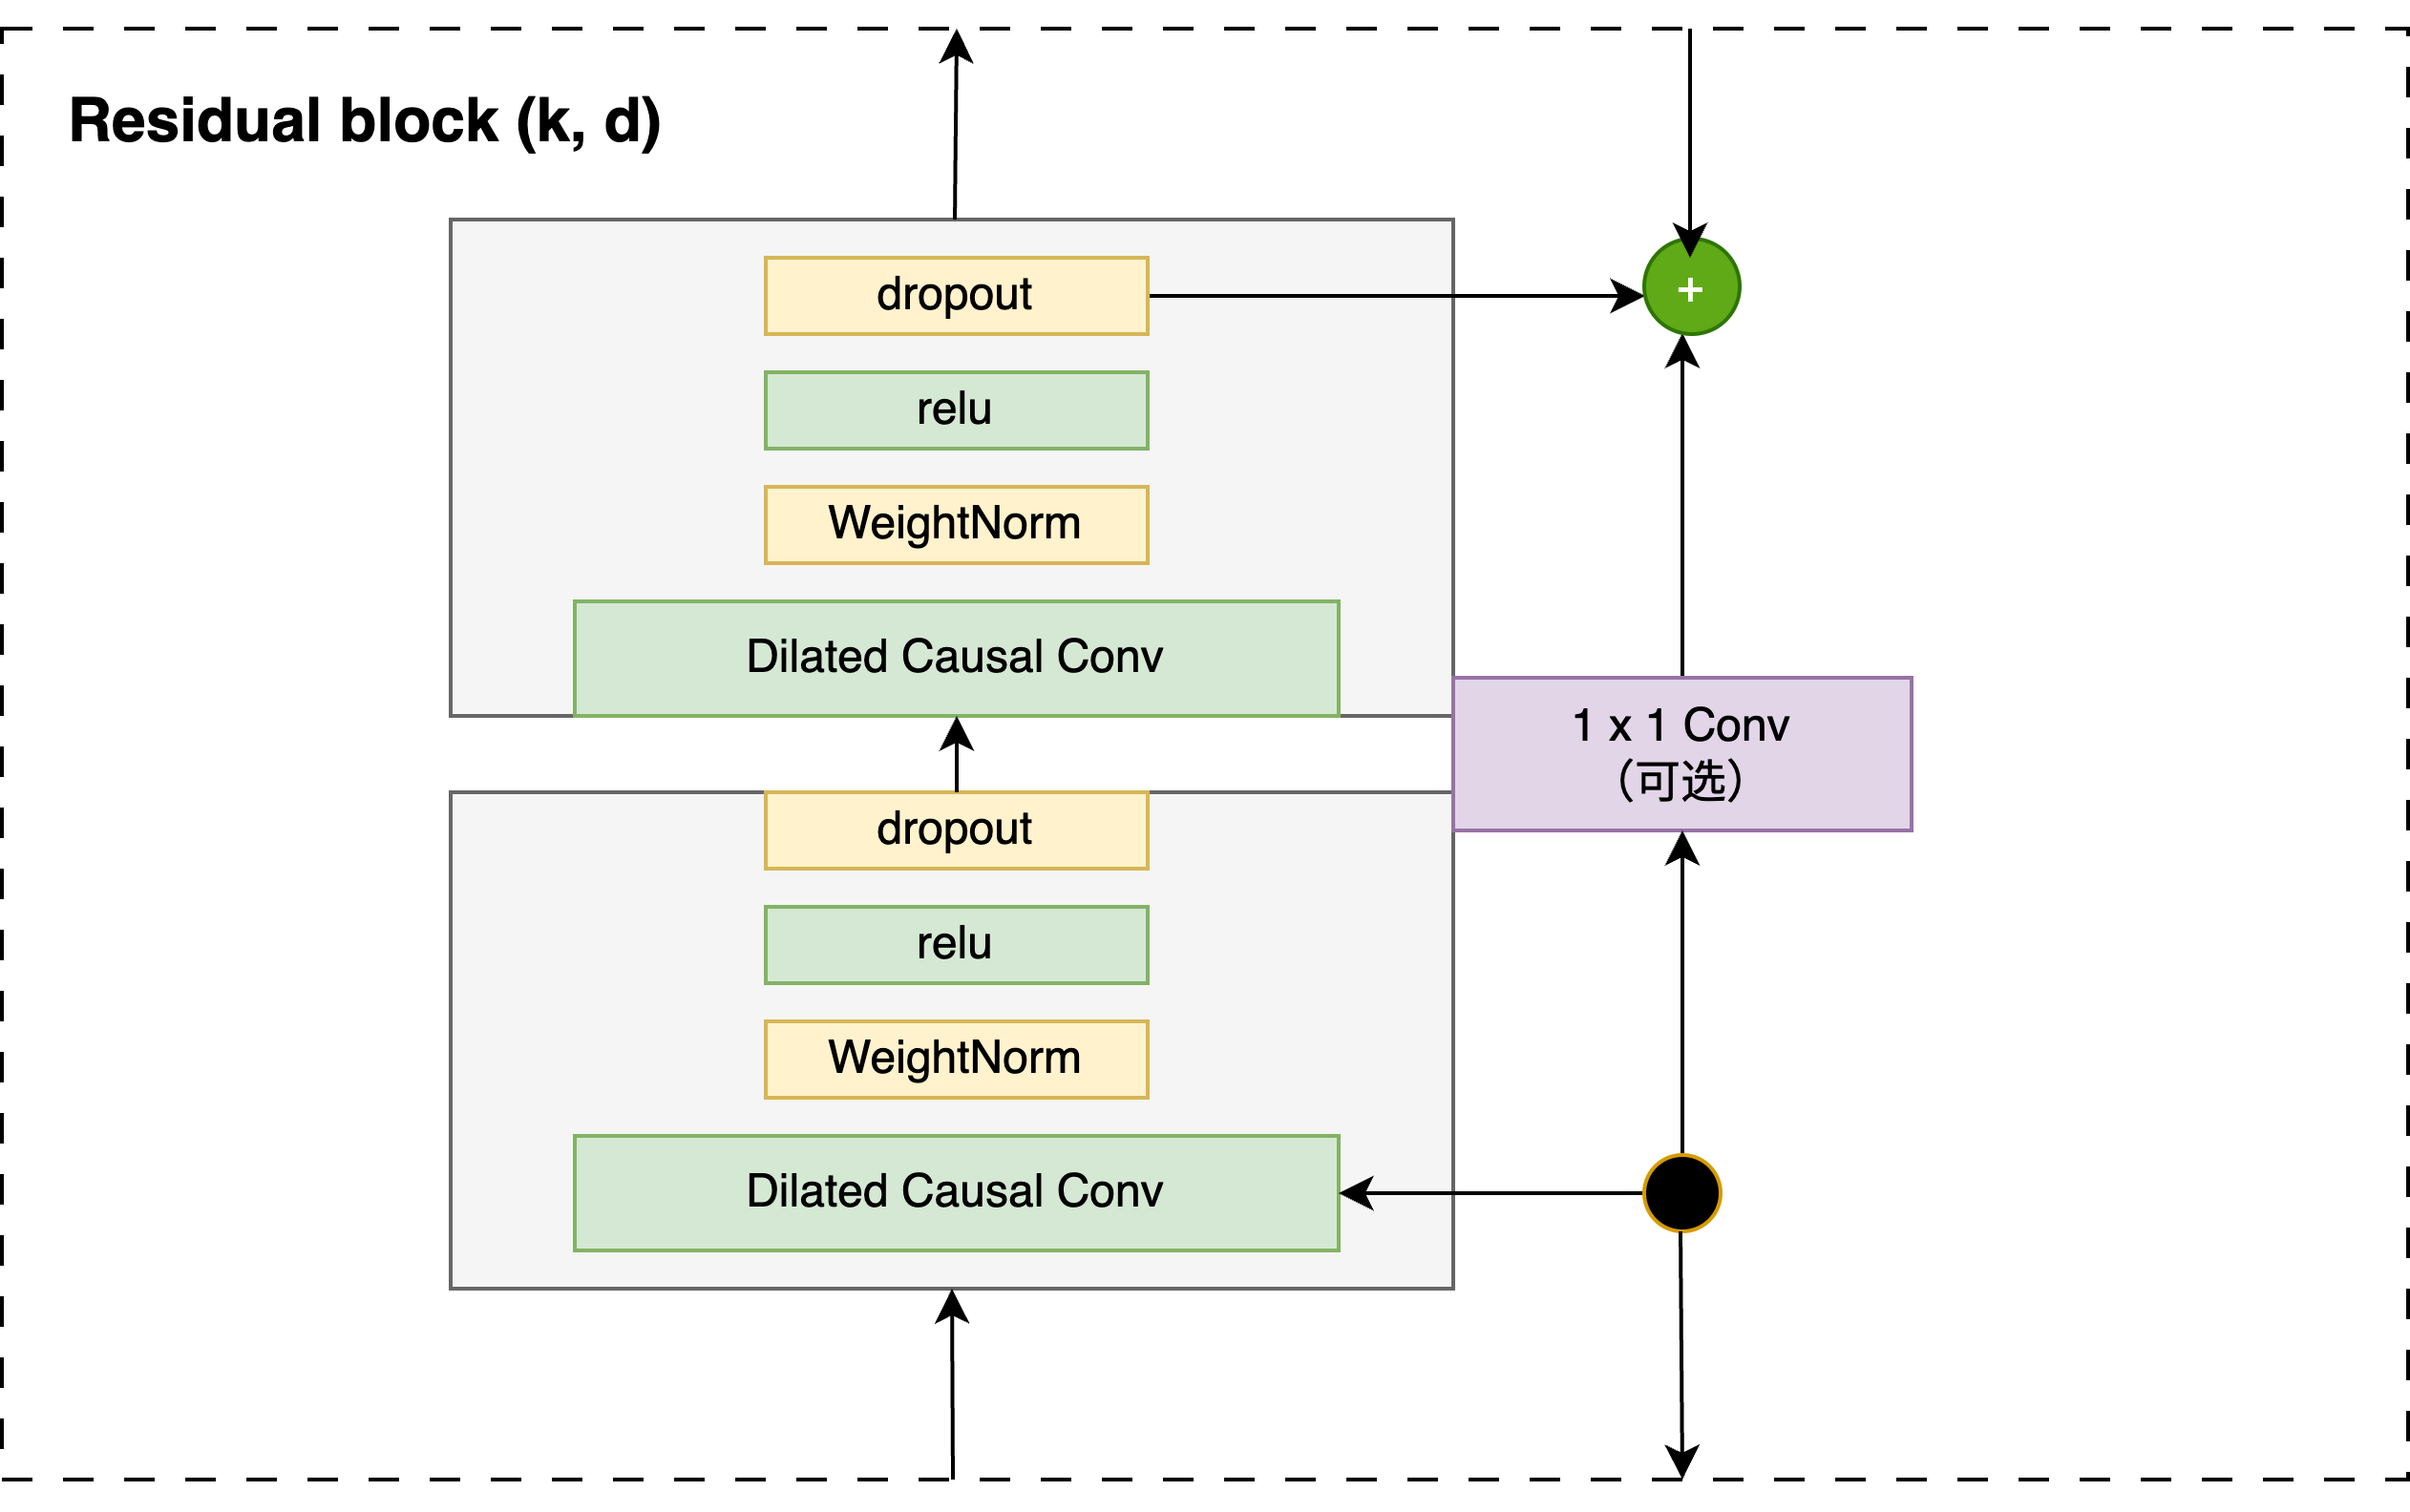
\includegraphics[width=\textwidth]{figures/resiual_tcn.png}
	\caption{TCN 的残差模块设计}
	\label{residual_tcn}
\end{figure}

于是整体的思路已经清晰,首先对时序数据集进行嵌入,嵌入使用指定大小的卷积核设置指定的膨胀因数,开始进行训练,进行归一向量化,和 ReLU 激活函数 Dropout 池化来防止梯度爆炸,最后用一个 Resnet 残差连接来避免梯度消失。

\section{时间卷积网络与负载情况的结合}
得到了综合负载评价指标和对应的时间就形成了一个常规的时间序列数据集,通过时间卷积网络深度学习即可较好的学习到时间序列内蕴藏的信息,通过蕴藏的信息预测未来的综合负载情况,返回给Nginx 集群内的负载均衡器,其以此来分配不同的不同的任务给空闲的服务器。

综合相关文献,对比了常规 RNN、LSTM、GRU 与 TCN 等循环神经网络在多种典型序列模型预测问题的性能表现上,结果表明 TCN 通常可以获得更好的预测精度,可以作为时间序列预测建模的有效手段\cite{bai2018empirical}\cite{赵洋2022基于时间卷积网络的短期电力负荷预测}。

(1)准备数据
通过使用监控脚本,周期性的收集 CPU、内存、磁盘 I/O 和网络带宽的利用率,并把这些数据保存到一个 CSV 文件中。由于作者本身的技能问题,不能使用高效率的监控程序,使用了 bash脚本来监控这些参数。

\begin{lstlisting}
#!/bin/bash

# 设置本地 CSV 文件路径
OUTPUT_FILE="/path/to/your/output_file.csv"

# 写入 CSV 文件的标题行
echo "Timestamp,CPU_Usage,Mem_Usage,Disk_Read,Disk_Write,Network_In,Network_Out" > $OUTPUT_FILE

# 设置网络接口名称
NETWORK_INTERFACE="eth0"

# 捕获信号,以便于退出
trap "echo 'Script terminated'; exit" SIGHUP SIGINT SIGTERM

# 开始收集数据
while true; do
    # 获取 CPU 使用率
    CPU_USAGE=$(top -bn1 | grep "Cpu(s)" | awk '{print $2 + $4}')

    # 获取内存使用率 (使用的内存比例)
    MEM_USAGE=$(free -m | awk 'NR==2{printf "%.2f", $3*100/$2 }')

    # 获取磁盘读写数据 (需要 sysstat 包安装)
    DISK_IO=$(iostat -dx | awk 'NR>3 {print $6,$7}' | awk '{read+=$1; write+=$2} END {print read,write}')

    # 获取网络带宽使用数据 (需要 ifstat 包安装)
    NETWORK=$(ifstat -i $NETWORK_INTERFACE 1 1 | awk 'NR==3 {print $6,$8}')

    # 获取当前时间戳
    TIMESTAMP=$(date '+%Y-%m-%d %H:%M:%S')

    # 写入数据到 CSV
    echo "$TIMESTAMP,$CPU_USAGE,$MEM_USAGE,$DISK_IO,$NETWORK" >> $OUTPUT_FILE

    # 设置延迟时间,例如每隔 1 分钟收集一次数据
    sleep 60
done
\end{lstlisting}

这个脚本会无限循环到直到我手动暂停,可以设置循环次数,也可以设置循环大周期,比如使用 nohup 来进行循环次数的限制,使用每日,每周,每月作为一个大周期获得较为长远的数据,来进行更加准确的预测。通过主成分空间分析得到的原始数据集,然后分为按照 $8:1:1$ 分为训练集、验证集和测试集。

(2)TCN 参数设置

由膨胀因果卷积的原理可知,TCN 模型中的扩大因子$d$ 和卷积核大小 $K$ 是决定TCN 模型预测性能的主要参数。
此参数的选择目前尚无理论指导, 一般均需通过实验对比取得\cite{hewage2020temporal}。
由于实验数据以及实验环境的限制,无法通过实验来确定当前不同配置的TCN模型的 $MAE$ 值和 $RMSE$ 值来确定最佳参数。
但是可以列举几个比较通用的模型参数,其中, 扩大因子 d 分别取值为 2、4 、8 和 16 ;卷积核 K 分别取为 1×3、1×5 和 1×7 ,两组参数共构成 12 种组合形式,如下表所示。

% \usepackage{tabularray}
\begin{longtblr}[
	caption = {TCN 模型参数组合},
	]{
	width = \linewidth,
	colspec = {Q[177]Q[158]Q[165]Q[183]Q[158]Q[160]},
	vline{4} = {-}{},
	vline{4} = {2}{-}{},
	hline{1,8} = {-}{0.08em},
		}
	序号 & $d$ & $K$ & 序号 & $d$ & $K$ \\
	1  & 2   & 1x3 & 7  & 8   & 1x3 \\
	2  & 2   & 1x5 & 8  & 8   & 1x5 \\
	3  & 2   & 1x7 & 9  & 8   & 1x7 \\
	4  & 4   & 1x3 & 10 & 16  & 1x3 \\
	5  & 4   & 1x5 & 11 & 16  & 1x5 \\
	6  & 4   & 1x7 & 12 & 16  & 1x7
\end{longtblr}

通过使用不同参数的 TCN 模型可以得到 MAE(平均绝对误差)即观测值与预测值绝对差的平均值、RMSE(均方根误差)即观测值与预测值差的平方的平均值的平方根。来确定最佳参数。 通过指定训练参数 epoch 以及 lr 来获得预测值,在通过与观测值的比较即可选择到较好的模型参数。

(3)特征学习训练以及优化网络模型

指定时间卷积的参数扩大因子$d$ 和卷积核尺寸$K$,以及指定的 epoch 和 lr 开始训练;使用均方根误差作为目标函数计算预估值和真实值的误差,并利用 Adam 优化算法更新网络中的参数\cite{kingma2014adam}。下面是重要的训练代码。

\begin{lstlisting}
# 定义均方根误差为损失函数
class RMSELoss(nn.Module):
    def __init__(self):
        super().__init__()

    def forward(self, yhat, y):
        return torch.sqrt(torch.mean((yhat - y) ** 2))

# 初始化损失函数
loss_function = RMSELoss()
# 开始进行训练
for epoch in range(num_epochs):
    for batch in train_loader:
        inputs, targets = batch
        optimizer.zero_grad()  # 清除过往梯度
        outputs = model(inputs)  # 获取模型预测结果
        loss = loss_function(outputs, targets)  # 计算损失
        loss.backward()  # 反向传播,计算梯度
        optimizer.step()  # 使用 Adam 更新模型权重
\end{lstlisting}

(4)输出预估值

在PyTorch中,可以直接调用模型对象并直接将输入数据传递给它以获得预测值。
\begin{lstlisting}
# 切换模型到评估模式
model.eval()

# 不计算梯度来加速计算和减少内存消耗
with torch.no_grad():
    for inputs in test_loader:
        # 输入新数据集
        predictions = model(inputs)
        # 输出预测值
        print(predictions)
\end{lstlisting}

在上述的代码中,prediction变量包含了模型基于inputs给出的预测结果。如果是预测未来一个时间步,prediction可能只是一个数字。如果是预测未来多个时间步,prediction可能是一个Numpy数组或者PyTorch张量,其中包含一系列预测值。如果输入的一条数据,那么输出的就是单一的预测值,如果输入的是一个序列,那么输出的就是包含多个值的序列。可以通过预测后的序列值观察综合负载情况,然后进行判断。

\section{本章总结}

本章首先探讨了如何获取到剩余性能的数据,并根据科学的主成分分析法来选取合适的权重参数,用合适的权重参数得到了能较好体现负载情况的综合负载指标数据集。

接着讨论了时间卷积网络与其他循环神经网络的不同之处,得到了其在时间序列预测性能的特征和具体原理和具体过程。最后将综合负载指标已经对应的时间戳形成对应的时间序列数据集。通过设置 epoch 和 lr 来暂时确定 MAE 和 RMSE 的走势情况,以获取训练的最佳参数。
设置了最佳参数后可以进行更大的 epoch 来实现更好的预测性能。总体描述使用时间卷积网络来进行训练的步骤,分化训练集和测试集,然后根据上面得到的最佳参数设置,进行网络训练拟合,最后输出我们想要的预估值。
